\chapter{Software}
\label{ch:software}

This chapter starts with a discussion on architecture, design, and
implementation aspects of the mobile app for the data collection.
Then, new features and changes in the \vadere\ simulation
software are described.
In preparation for this work, many changes and enhancements were necessary,
which are documented in the following sections.
The last three sections present a tool to generate train scenarios, the seating
model's implementation, and the subsystem used for model verification.

\section{Mobile app for data collection}

In chapter~\ref{ch:data}, requirements for an data collection app are gathered and
the resulting app is introduced.
This section describes design and implementation of this app.

\subsection{Software design}

This section describes some interesting aspects of the app's software design.

\subsubsection{Actions}

To conduct the survey, the \acsp{UI} in figure~\ref{fig:app-screen-3}
and~\ref{fig:app-screen-4} (section~\ref{sec:mobile-app}) provide a number of actions.
Examples for these actions are logging of events (``sit down'', ``leave'',
etc.) and assigning properties to persons (age, gender).
Requirements related to the actions are:

\begin{itemize}

  \item The actions must be undoable to allow for correcting mistakes.

  \item There is a type of actions that requires further user action.
    For example, for defining a group of persons, the action is started but not
    finished before the members are selected.
    These actions are called pending actions and they all have in common that
    the user have to select seats to finish the action.

  \item For pending actions, there must be a way to notify the \acs{UI} when the
    action has been finished or canceled. For example, the \acs{UI} might have
    to change some icon color back to its default.

\end{itemize}

To implement the actions and requirements, I use a pattern similar to the Java
Swing
\href{https://docs.oracle.com/javase/8/docs/api/javax/swing/undo/UndoManager.html}{\code{UndoManager}}
(which is not available on Android). Each type of
action has its own class and all actions are carried out by an
\code{ActionManager} object. Figure~\ref{fig:uml-class-diagram-actions} shows an
simplified \acs{UML} class diagram of this design.

The actions need a reference to the action manager because some of them have to
perform subsequent actions and others have to interact with the \acs{UI}, which
is only available through the action manager.

\begin{figure}[htb]
  \centering
  \includegraphics[width=14cm]{uml-class-diagram-actions}
\caption[\acs{UML} class diagram of actions.]%
{\acs{UML} class diagram of the action manager, actions, and pending actions.}
\label{fig:uml-class-diagram-actions}
\end{figure}

All related classes reside in the Java subpackage \code{.actions};
see section~\ref{sub:app-dev} for more technical details.

\subsubsection{Model and database schema}
\label{subsubsec:model-and-db-schema}

With the library Sugar ORM, I use \acf{ORM} for database access.
\acs{ORM} is a technique to access a database from an object-orientated
programming language using objects that correspond to the database entities.

In the case of Sugar ORM, the database scheme is primarily defined through Java
classes, which describe the database entities.
These classes reside in the Java subpackage \code{.model} and they are
subclasses of \code{SugarRecord}.

In the following I use the terms \emph{entity class} for the correspondents of
database entities and \emph{model class} for classes used as model behind the app's
view (in terms of \acs{MVC}).

Model and entity classes are almost identical.
However, model classes have some properties that are only relevant for the
running app but should not be persistent.
To solve this problem there are a number of possible solutions:

\begin{enumerate}

  \item The model class can be a subclass of the entity class.
    In this case, the entity objects cannot directly be reused for the model
    objects---data must be copied to new model objects.

  \item The model objects can store a reference to their corresponding entity
    objects.

  \item Entity and model class can be the same class as long it is guaranteed
    that model-only properties are not persisted.
    This is technically possible with Sugar ORM by applying its Java annotation
    \code{@Ignore} to these properties.

\end{enumerate}

I implemented the last option: Shared classes for entities and model.
This keeps the total number of classes low and does not require copying data or
managing extra objects.

Figure~\ref{fig:uml-class-diagram-model} illustrates the simplified model.
The container class for seats, which defines the seating layout, is left out
because it is more related to the \acs{UI}.
Classes that are also entity classes are marked with \flqq{}entity\frqq.
On the class \code{Person} (in the center), there are a few things to note:

\begin{itemize}

  \item The properties \code{agent} and \code{disturbing} should not be
    persisted---they are ignored by the \acs{ORM} library (\code{@Ignore}
    annotation).
    The property \code{agent} specifies whether the person is the investigator
    conducting the survey.
    This information is already stored in the survey entity object.
    The property \code{disturbing} specifies whether the person is currently
    disturbing.
    Because this can change over time, it is saved as a log event, instead.
    Still, both are properties of the person object and both are required as
    state information for the \acs{UI}.

  \item With the property \code{mGroup} persons can be assigned to a group of
    friends or colleagues. This might be interesting to observe seating behavior
    of groups. The ``M'' in the entity class name \code{MGroup} can be
    interpreted as ``mates'' or ``model''. The name \code{Group} could not be
    used because of a bug in the \acs{ORM} library.\footnote{A class named
      \code{Group} produces an error in the current version of Sugar ORM because
      \code{GROUP} (case-insensitive) is a reserved keyword in \acs{SQL}.
      This is a bug and there is an open issue on this:
      \url{https://github.com/satyan/sugar/issues/98}}

  \item The properties \code{gender} and \code{ageGroup} are enums.
    Both enums have a special \NA\ value for \acf{N/A}.
    This way I can directly use the enums as the data source for the
    \href{https://developer.android.com/guide/topics/ui/controls/spinner.html}{Android
    Spinner components}, which allow the user to select a value from a list.
    Otherwise I would have to hard-code the values or provide an extra
    wrapper class which adds an \acs{N/A} value.
    To assure that the properties cannot be \code{null}, they have the
    \code{@NotNull} annotation.

\end{itemize}

\begin{figure}[htb]
  \centering
  \includegraphics[width=14cm]{uml-class-diagram-model}
\caption[\acs{UML} class diagram of the app's entity model.]%
{This is an \acs{UML} class diagram of the app's entity model.}
\label{fig:uml-class-diagram-model}
\end{figure}


\subsubsection{Android Fragments}

\href{https://developer.android.com/reference/android/app/Fragment.html}{Android
Fragments} are reusable portion in an
\acs{UI}.\footnote{\url{https://developer.android.com/guide/components/fragments.html}}
They gather \acs{UI} controls and behavior in a self-contained form.

The app's main \acs{UI} portion is the seating layout which represents the
current state of the data collection (seats, persons, baggage, \ldots).
This part is self-contained and it is required twice in the app: for the
initialization phase and during the data collection.
Therefore it is implemented as a fragment in the class \code{SeatsFragment}.
As a fragment, it takes parameters:

\begin{itemize}

  \item A survey object that holds the meta data of the survey (date, train
    line, direction, \ldots).

  \item An optional \code{SeatsState} object that holds the state for
    initializing the fragment.
    This parameter is used to pass the initial state to the next screen
    (figure~\ref{fig:app-screen-3} and~\ref{fig:app-screen-4}).
    If it is missing, all seats are initialized empty.

  \item The train direction.
    It is visualized with an arrow and part of the fragment's internal state.

\end{itemize}

Fragments are also used to define dialog \acsp{UI}, \eg the dialog to set and
update person properties.

\subsubsection{Database export to \acs{CSV}}

For further data analysis, I need plain-text \acs{CSV} files on the computer.
Therefore, the app must be capable to export its database tables to \acs{CSV}
files and save these files to the phone's storage.
The phone can then be connected to the computer and the files can be copied.

Database export and file \acs{I/O} can be a demanding and time-consuming
operation.
To not freeze the \acs{UI} during the export process, I use an
\href{https://developer.android.com/reference/android/os/AsyncTask.html}{Android
AsyncTask}, which starts a thread in the background.
The following listing shows the entry-point to the export implementation.
The method's signature is specified by the \code{AsyncTask} class.

\lstinputlisting[%
language={java},%
caption={Entry-point method to the database export.},%
label={lst:db-export}]%
{listings/db-export.java}

The following methods are called during the export
process:\footnote{\verb~grep 'private .*(.*)' seating-datacollection/**/DatabaseExportTask.java~\shellcmdline}

\begin{itemize}
  \item \code{private void exportAllTables()}
  \item \code{private List<String> getTableNames()}
  \item \code{private void exportTable(SQLiteDatabase db, String tableName, File directory)}
  \item \code{private Cursor queryTable(SQLiteDatabase db, String tableName)}
  \item \code{private String[] getFieldsAsStringArray(Cursor cursor)}
\end{itemize}

Two problems arose during implementing the database export:

\begin{enumerate}

  \item The Android \acs{API} for saving files does not work consistently.
    Android can save files to internal and external
    storage.\footnote{\url{https://developer.android.com/training/basics/data-storage/files.html}}
    Files saved to the internal storage are only accessible by the app.
    Therefore, when exporting files, the external storage must be used.
    The development device, a Nexus~6 smartphone, does not have an SD card.
    Thus, the \acs{API} call
    \href{https://developer.android.com/reference/android/os/Environment.html#getExternalStorageState()}{Environment.getExternalStorageState()}
    yields a state other than the required
    \href{https://developer.android.com/reference/android/os/Environment.html#MEDIA_MOUNTED}{Environment.MEDIA\_MOUNTED}.
    Despite of this result, the concept of external storage exists on a Nexus~6
    and files can be saved into paths returned by
    \href{https://developer.android.com/reference/android/os/Environment.html#getExternalStorageDirectory()}{Environment.getExternalStorageDirectory()}
    and similar methods.
    This inconsistency seems to be an Android problem because there is no other
    \verb|MEDIA_*| state for the case of Nexus~6 and the official guide on
    data-storage (referenced above) does not mention this problem as of
    2016-08-15.

  \item Exported files are not visible to the computer until the phone is
    restarted.
    The Nexus~6 device can be connected to the computer using the \acf{MTP}.
    This is the only mode that allows users to access the phone's storage.
    While the exported files are visible in the device's file manager app, they
    are initially \emph{not} visible (and subsequently not up-to-date) to the
    computer.
    According to \citep{Manua66:online}, this is because no media scan is
    triggered when files are saved to external storage, despite I am using the
    standard \acsp{API}.
    I tried different default folders (\code{Documents}, \code{Download},
    \ldots) as well as the root folder of the external storage---they all have
    the same problem.
    The source mentioned above lists a number of ways to initiate a media scan.
    Some ways do not apply for the development device as it is not rooted and it
    does not have CyanogenMod\footnote{\url{http://www.cyanogenmod.org/}}
    installed.
    Other ways do not work \eg making a photo to trigger a media scan or start
    the scan programmatically.
    This is the only work-around I have found so far: Restart the phone after
    each database export before copying the files to the computer.

\end{enumerate}

\FloatBarrier

\subsection{App development}
\label{sub:app-dev}

Here are some technical details on the app development.

\begin{table}[h]
  \begin{tabular}{ll}
    \hline
    Target Platform           & Android                                        \\
    Target \acs{SDK} version  & 23                                             \\
    Minimum \acs{SDK} version & 21                                             \\
    \acs{IDE}                 & Android Studio 2.1.2                           \\
    Development platform      & Arch Linux                                     \\
    Development device        & Motorola Nexus~6, Android 6.0.1                \\
    App name                  & \code{SeatingDataCollectionApp}                \\
    App package               & \code{edu.hm.cs.vadere.seating.datacollection} \\
    \hline
  \end{tabular}
\caption{Table of technical details on the app development.}
\label{tab:app-dev}
\end{table}

For the development of the Android app, I used Google's Android Studio 2.1.2.
It is ``The Official IDE for
Android''\footnote{\url{https://developer.android.com/studio/} (accessed:
2016-08-09)} and it has very good support for the Android \acs{SDK}.

The app has the following library dependencies, defined in the Gradle build
file:\footnote{\verb~grep ' compile ' seating-datacollection/SeatingDataCollection/app/build.gradle~\shellcmdline}

\begin{itemize}[noitemsep]

  \item Sugar~ORM, version~1.5 for \acf{ORM} between the SQLite database and
    Java objects.

  \item opencsv, version~3.7 for export from the SQLite database to \acs{CSV}.

\end{itemize}

This app is open-source, available under the GPL v3 license, and hosted at
GitHub: \url{https://github.com/schoettl/seating-datacollection}

\subsection{Evaluation of a different approach}

Before I committed to implement the mobile app for data collection, I evaluated
a different approach using plain text files together with a programmable text
editor\footnote{In this section, ``editor'' refers to a text editor. Notepad++,
VIM and GNU~Emacs are examples for text editors.} and shell scripts.
This idea seemed promising because of two main reasons.

First, there are some required features that an editor like VIM or Emacs already
has built in.
In contrast, in an app, these features must be implemented again.
Some of these features are quick selection of \acs{UI} elements, support for
multiple concurrent views, undo and redo capabilities, and facilities to correct
the event log.

Second, the collected data are finally required in plain text \acs{CSV} files for
further analysis.
An editor is predestined for handling these files.
In contrast, an app would use a database and would export the \acs{CSV} files later
which then must be transferred to the computer.

I chose the editor VIM as the platform and prototyped a tool for data
collection according to the requirements described in
section~\ref{sec:data-requirements}.
A rough description of the software architecture follows below.
Advantages, drawbacks and reasons why I stopped following this approach are
listed next.

\subsubsection{Architecture}

The architecture consists of the following components:

\begin{itemize}

  \item Plain text \acs{CSV} files for data.
    These files get appended during data collection and can later directly be
    used for data analysis and statistics.

  \item Plain text files representing the \acs{UI}.
    These template files are copied at the beginning of the data collection and
    then displayed in the editor.
    Together with the editor, they form the \acl{UI}.

  \item Shell scripts as controller component.
    A few shell scripts act as a controller.
    To start a data collection, the script \code{start-survey.sh} is invoked
    at the command line. This starts the editor with the \acs{UI}. Another shell
    script converts the current state of the \acs{UI} (a plain text file) into
    one or more lines and appends them to the data \acs{CSV} files.

  \item Configuration and shortcuts in the editor to make the \acs{UI}
    interactive.
    The editor must be tweaked to enable or trigger certain actions.
    For example, a keyboard shortcut has to be configured, to invoke the shell
    script that writes the current state to the data \acs{CSV} files.

\end{itemize}

Figure~\ref{fig:seatingdatacollection-vim-ui} shows a screenshot of the main
\acs{UI} from a prototype.

Regarding usage efficiency, performing actions in the editor approach is
comparable to a touch \acs{UI} of a mobile app.
However, it cannot be denied that learning how to use an editor like VIM
efficiently, is a long way to go.
As an example, to position the cursor to enter the age group for the person
sitting on seat ``a'' (see figure~\ref{fig:seatingdatacollection-vim-ui}), only
four key strokes on a computer keyboard are required\footnote{\verb|`a3j|,
  provided that the seats have a cursor mark.}.

\begin{figure}[htb]
  \centering
  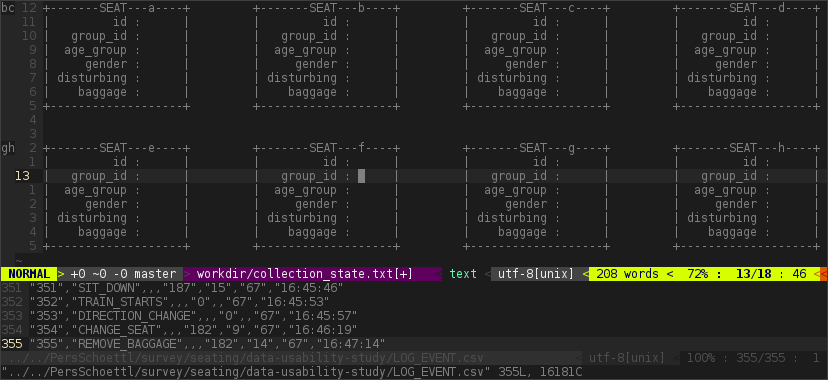
\includegraphics[width=14cm]{seatingdatacollection-vim-ui}
  \caption[Prototype of a user interface for data collection using VIM.]%
  {Prototype of a user interface for a data collection using VIM and shell
  scripts.}
\label{fig:seatingdatacollection-vim-ui}
\end{figure}

\subsubsection{Advantages}

There are technical and personal reasons speaking for the editor approach.

One important technical aspect is the database.
In Android this includes a relational database structure, database connection
and version management, entity classes, \acf{ORM}, \aclp{UI}, and export to
\acs{CSV} files on the external storage.
These are many technical challenges, though ultimately I only need the
exported \acs{CSV} files for data analysis.
In contrast, the editor approach operates directly on the final data files.
This allows for simple appending of new lines and precise corrections.
Using an editor, this comes without any of the challenges mentioned above.

Another reasons is my preference for reusing existing functionality instead of
reimplementing it in an mobile app.
Here is a list of some features that already exist in the editor:

\begin{itemize}

  \item Split windows to tile the screen into different areas are an integral
    part of VIM.
    One window could show the main \acs{UI} while other windows could
    show the data files for monitoring and corrections.

  \item Undo and redo is built-in in editors like VIM.
    This makes it easy to undo mistaken inputs---in the \acs{UI} displaying the
    seats as well as in the data files.

  \item Automatic reload of data files, when they get appended through the
    \acs{UI}, is just a configuration option.

\end{itemize}

Finally, a personal reason for first looking for another approach is this:
I have never designed or developed a mobile app before.
Having an app with custom widgets, reusable components, context and option
menus, support for undoing actions, database with abstraction layer, and file
export is not trivial and maybe not the best way to learn Android programming.

\subsubsection{Drawbacks}

During the evaluation phase, some problems and difficulties with the editor
approach came up.

\begin{itemize}

  \item The \acs{UI} text file (see
    figure~\ref{fig:seatingdatacollection-vim-ui}) must be converted to a line
    of \acs{CSV} to get appended to the data file.
    There are simple ways to parse the text file and get the required data,
    using tools like AWK, but this is not robust against slight mistakes in the
    \acs{UI} text file.
    For example, if the user inadvertently uses a pipe symbol (\code{|}) in the
    text, the conversion might give incorrect or corrupted results.

  \item For many \acs{UI} actions, the number of the seat, where the cursor is
    positioned, is required.
    To get the seat number from the cursor position, rectangle coordinates have
    to be defined;
    either by hard-codeding them or by parsing the \acs{UI} text file.
    Parsing has the same problems as described in the previous paragraph.

  \item Users can only work with the program if they have a high experience with
    VIM. This means, that very few people interested in this kind of data
    collection, can actually reuse the program.

\end{itemize}

Therefore---despite the advantages of using VIM with plain text files---I
decided to move on with the mobile app development.

\section{\vadere\ crowd simulation}

\vadere\ is an open source framework for the simulation of microscopic
pedestrian dynamics \citep{vadere2016:online}.
It has been developed by Prof.\,Dr.\ Gerta Köster's research group at the
\acl{MUAS}.

\vadere\ facilitates the development of new simulation models that can be
implemented in stand-alone Java classes and then be linked into the simulation
framework.
This promotes research in the field of pedestrian dynamics and enables the use
for educational purpose \citep{seitz-2016}.
Beside pedestrian dynamics, \vadere\ can also be used for simulation of traffic
systems or particle systems.

In August 2016, \vadere\ was released as an open source project under the
terms of the \href{http://www.gnu.org/licenses/lgpl.html}{GNU LGPL}.
Its Git repository is hosted at a GitLab instance and can be found at:
\url{https://gitlab.lrz.de/vadere/vadere}

\section{Contributions to \vadere}

\subsection{Source controller}
\label{sec:source-controller}

During a simulation, pedestrians are created (spawned) at certain spots in
the scenario called sources.
This process is controlled by source controller instances.
I rewrote most parts of the source controller to enable spawn distributions
(see section~\ref{sec:spawn-distributions}) and a maximum number of pedestrians to
be spawned.

The following Java classes are involved in the implementation:

\begin{itemize}

  \item \code{Source}---An object of this class represent a source where
    persons are spawned.
    All parameters are stored in the instance variable \code{attributes}, which
    is of the class \code{AttributesSource}.

  \item \code{AttributesSource}---An object of this class represent static
    parameters for a source.
    These parameters include an \acs{ID}, a shape, and a start and end time
    amongst others.
    Objects of this class can be serialized to and deserialized from \acs{JSON}.
    This way, the parameters can be configured via \acs{JSON}, \eg in the
    \acs{GUI}.

  \item \code{SourceController}---An object of this class has a source
    associated and actually creates and spawns new persons according to the
    source's parameters.

  \item \code{TestSourceController*}---These are unit tests for the
    \code{SourceController} class.

\end{itemize}

Originally, sources were designed to spawn persons only with a configurable
constant rate.
This is an example \acs{JSON} configuration for the sources before distributions
were introduced:

\begin{lstlisting}[%
language={},% JSON and JavaScript are not supported :(
caption={[Example configuration without spawn distribution.]%
  An example configuration for sources before distributions were introduced.},%
label={lst:old-source-config}]
{
  "startTime": 10,
  "endTime": 15,
  "spawnDelay": 1,
  "spawnNumber": 2,
  ...
}
\end{lstlisting}

This source starts with spawning persons at $10 \si{\second}$ of simulation
time.
Until $15 \si{\second}$ (inclusive), every $1 \si{\second}$, 2 persons are
created.

\subsubsection{The \code{SourceController} class}

The \code{SourceController} class contains all the logic of spawning
pedestrians.
This class was largely rewritten to support the new features.
The algorithms are implemented according to the principles of Clean
Code \citep{martin2009clean} where readability and maintainability are main
goals.

During the implementation of spawn distributions and the maximum spawn number, I
extended the existing unit test class of the \code{SourceController} class and
added new test methods.
This way I can thoroughly test new functionality while making sure that my
changes do not break existing tests.

\subsubsection{Design and implementation of spawn distributions}
\label{subsec:design-impl-spawn-distributions}

In the following, I introduce a new design using spawn distributions to overcome
the limitations of \code{spawnDelay}.

In the class \code{AttributesSource}, the field \code{spawnDelay} is deleted in
favor of two new fields and one constant:

\lstinputlisting[%
language={Java},%
caption={New fields for spawn distribution in class \code{AttributesSource}.},%
label={lst:source-attributes-fields-spawndistribution}]%
{listings/attributessource-spawndistribution.java}

The field \code{interSpawnTimeDistribution} is the fully-qualified class name of
a distribution class.
Distribution classes must fulfill two requirements:

\begin{enumerate}

  \item They must implement the interface
    \href{https://commons.apache.org/proper/commons-math/javadocs/api-3.6.1/org/apache/commons/math3/distribution/RealDistribution.html}%
      {\code{org.apache.commons.math3\-.distri\-bution\-.Real\-Distribution}}
    from the Apache Commons Math
    library\footnote{\url{https://commons.apache.org/proper/commons-math/}}.
    The library also provides a wide range of standard distributions that can be
    used.

  \item They must provide a public constructor with the following parameters:
    The first parameter must be an
    \href{http://commons.apache.org/proper/commons-math/javadocs/api-3.6.1/org/apache/commons/math3/random/RandomGenerator.html}%
      {\code{org.apache.commons.math3.random\-.Random\-Generator}}.
    Further constructor parameters make up the distribution's parameters.
    They are all of type
    \href{https://docs.oracle.com/javase/7/docs/api/java/lang/Double.html}%
      {\code{java.lang.Double}}.
    The distributions can have any number of parameter.
    Only the \code{RandomGenerator} is mandatory.

\end{enumerate}

The field \code{distributionParameters} defines the list of distribution
parameters.
Its length must match the number of \code{Double} parameters in the
distribution's constructor.

The default spawn distribution is the constant distribution, which has the same
effect as \code{spawnDelay} before.

For the train scenario, I can now use the distribution
\href{https://commons.apache.org/proper/commons-math/javadocs/api-3.6.1/org/apache/commons/math3/distribution/ExponentialDistribution.html}%
  {\code{org.apache.commons\-.math3\-.distribution\-.ExponentialDistribution}}
with the parameter $λ$ calculated in section~\ref{sec:spawn-distributions}.

\subsubsection{Implementation of a maximum spawn number}

There is another minor issue to be addressed: How to spawn a fixed number of
pedestrians?
This was possible before, \eg to spawn two pedestrians, the parameters would
have been: \code{startTime = 1, endTime = 2, spawnDelay = 1}.
However, with spawn distributions, the time between two spawn events is not
fixed anymore but random.
Therefore, setting the end time is not applicable.

A solution is to add a another field to the \code{AttributesSource} class:

\lstinputlisting[%
language={Java},%
caption={New field for maximum spawn number in class \code{AttributesSource}.},%
label={lst:source-attributes-field-maxspawnnumbertotal}]%
{listings/attributessource-maximumspawnnumbertotal.java}

This parameter controls the maximum number of pedestrians that can be spawned.
The default value zero means, that there is no maximum.
Now, to spawn a fixed number of pedestrians,

\begin{enumerate}[noitemsep,nolistsep]

  \item \code{maxSpawnNumberTotal} is set to the desired number, and

  \item \code{endTime} is set to a large value, \eg \code{10e9} (1,000,000,000).

\end{enumerate}

While in theory, the end time can still be the limiting factor, this is a direct
and pragmatic solution, which does not require any changes in any existing
scenario definitions.
Listing~\ref{lst:new-source-config} shows an example of how this attribute can
be used.

\subsubsection{Example usage}

For example, a source can now be configured like this:

\begin{lstlisting}[%
language={},% JSON and JavaScript are not supported :(
caption={An example configuration for sources with a spawn distribution.},%
label={lst:new-source-config}]
{
  "startTime": 10,
  "endTime": 100,
  "maxSpawnNumberTotal": 5,
  "interSpawnTimeDistribution": "org.apache.commons.math3.distribution.UniformRealDistribution",
  "distributionParameters" : [ 1, 3 ],
  ...
}
\end{lstlisting}

The two distribution parameters \verb|[ 1, 3 ]| are the lower and upper limit of
the uniform distribution.
It can be looked up in the
\href{https://commons.apache.org/proper/commons-math/apidocs/}%
{Apache Commons Math API documentation} for the respective distribution.

\subsection{Target controller}

During a simulation, pedestrians are moving towards their individual targets.
If they have no target, they do not move.
If they have multiple targets, they move from one target to the next one in the
order specified in their target list.

Targets are certain spots in the scenario and they have a variety of properties.
For example, it can be defined if pedestrians are ``absorbed'' when they reach
the target or if they continue to live in the scenario.

For each target, there is a target controller which handles the case when a
pedestrian reaches its target.
The following classes are related to the implementation of targets:

\begin{itemize}

  \item \code{Target}---An object of this class represent a target.
    All its static properties are stored in an instance variable of type
    \code{AttributesTarget}.

  \item \code{AttributesTarget}---An object of this class defines all static
    parameters of a target.
    The parameters include an \acs{ID}, a shape, and the ``absorbing'' property
    mentioned above.
    Attributes objects can be serialized to and deserialized from \acs{JSON}.
    This is the way how targets are configured, \eg in the \vaderegui.

  \item \code{Agent}---An object of this class represents a
    pedestrian.\footnote{To be precise, there is a subclass \code{Pedestrian}
    but this subclass does not add any properties relevant for this section.}
    A pedestrian (as an agent) has a target list which stores the pedestrian's
    targets in the correct order.
    A pedestrian also has methods to access the target list and get the current
    target.

  \item \code{TargetController}---For each target, there is one target controller.
    The target controller detects when a pedestrian reaches its target and
    handles that event.
    The process of handling that event includes:

    \begin{itemize}[noitemsep,nolistsep]
      \item The controller removes the pedestrian from the scenario if the
        target is absorbing.
      \item If the target is not absorbing, the controller updates the
        pedestrian's current target according to the pedestrian's target list.
    \end{itemize}

  \item \code{Potential\-Field\-Target}---Subclasses of this interface implement
    floor fields for navigation \citep{kirik-2007,kirik-2009,koster-2014b}.

\end{itemize}

Beside a lot of refactoring in these classes, I corrected the design of the
target list and implemented an observer pattern \citep{gamma-1995} to notify
clients about events at targets.

\subsubsection{Pedestrian's target list}

Initially a pedestrian's target list was a queue.
The current target was always the first one in the queue and it was popped when
a pedestrian had reached this target.
New targets could be added to the end of the queue.

Some simulation models, however, required to query or switch back to previous
targets.
Some effort was made to change the queue to a list and introduce an index
variable which points to the current target.
This implementation was incomplete and did not provide a clean interface.

I corrected the design and the implementation of the target list.
The affected classes were mainly \code{Agent}, \code{TargetController},
\code{Potential\-Field\-Target}, and its subclasses.
The updated \acs{API} propagated into most simulation models, simplifying code
and logic therein.

The class \code{Agent} now provides the following methods to work with the
target list:

% TODO change Next to Current (when it is changed in code)
\begin{itemize}

  \item \verb|boolean hasNextTarget()|
    \\
    Queries if the pedestrian currently has a target.

  \item \verb|int getNextTargetId()|
    \\
    Gets the \acs{ID} of the pedestrian's current target.
    This method throws an exception if the pedestrian currently has no target.

  \item \verb|List<Integer> getTargets()|
    \\
    Gets the list of the pedestrian's target \acsp{ID}.
    This list can be modified or new targets can be added.

  \item \verb|void incrementNextTargetListIndex()|
    \\
    Increments the index which points to the pedestrian's current target so that
    it points to the next target in the list.

  \item \verb|void setNextTargetListIndex(int nextTargetListIndex)|
    \\
    Sets the index which points to the pedestrian's current target.

  \item \verb|int getNextTargetListIndex()|
    \\
    Gets the index which points to the pedestrian's current target.

\end{itemize}

The methods in this list are ordered by importance.
The first methods are used most frequently.

\paragraph{Details}

Beside simulation models, the target controller and the
\code{Potential\-Field\-Target} classes use this \acs{API}.

The target controller checks its target area for pedestrians and processes the
``target reached'' program for pedestrians that have a matching target.
The methods \code{hasNextTarget} and \code{getNextTargetId} are used to compare
the controller's target with the pedestrian's target.
If the target is not absorbing, the controller uses the method
\code{incrementNextTargetListIndex} to update the pedestrian's target.

The \code{PotentialFieldTarget} classes implement potential floor fields which
are used to navigate pedestrians towards their targets.
They have two methods to get a potential value and a potential gradient at a
specific point related to a specific target.
Previously, the parameters for this methods were the position, the pedestrian,
and the target list (which was redundant).
Now, only the position and the pedestrian are passed as arguments.
The implementations use the methods \code{hasNextTarget} and
\code{getNextTargetId} to get the target.

\paragraph{Backwards compatibility}

For backward compatibility, the target list can still be used as a queue.
Code for compatibility is marked as deprecated and it is well separated from the
new implementation so that it can eventually be dropped easily.

Backward compatibility can be enabled by calling
\verb|setNextTargetListIndex(-1)| (or specifying this value in the \acs{JSON}
configuration).
In this mode, the methods defined above treat the target list as a queue.
For example, \code{getNextTargetId()} always returns the first target in the
list.

\subsubsection{Target listener}
\label{subsec:target-listener}

With target listeners, I implemented a way to inform clients about events that
occur on targets, \eg when a pedestrian reaches its target.
The implementation's design is based on the Observer pattern.

Before I implemented that feature, when a client wanted to know if a pedestrian
reached its target, the client had to compare the pedestrian's position and
target at every simulation step.
Many clients implemented this polling algorithm which led to redundant and
error-prone code and an inefficient simulation loop.

Target listeners provide a more event-driven way.
A client can register its listener(s) on a target.
The target controller notifies the registered listeners about events.

Listing~\ref{lst:target-interface-for-listener} shows the related methods in the
\code{Target} class.
The \code{TargetController} class has the method
\code{notifyListenersTargetReached} to notify registered listeners when a
pedestrian has reached its target.
Currently, only this event type is supported but other event types can be added
easily.

\lstinputlisting[%
language={Java},%
caption={The \code{Target} class' interface for working with target listeners.},%
label={lst:target-interface-for-listener}]%
{listings/target-interface-for-listener.java}

Target listeners are used in the seating model
(section~\ref{sec:model-implementation}) and in the data processor for its
verification (section~\ref{sec:model-verification}) as well as in other
simulation models and data processors.

\subsection{Model framework redesign}
\label{sec:simulation-model-framework}

During the preparations of releasing \vadere\ as open source, we redesigned the
way how simulation models are defined.

Simulation models implement the logic of a model and are often hooked into the
simulation loop.
Examples for such models are the \osm\ \citep{seitz-2012,seitz-2016}, the floor
field models, and the seating model.

Requirements are that it must be possible to configure the models in \acs{JSON}
and to combine independent models without having hard dependencies in the code.

\subsubsection{Resulting design}

\begin{figure}[htb]
  \centering
  \includegraphics[width=8cm]{model-framework}
  \caption[Simplified \acs{UML} class diagram of simulation model framework.]{%
  Simplified \acs{UML} class diagram of the simulation model framework.
  }\label{fig:uml-model-framework}
\end{figure}

Figure~\ref{fig:uml-model-framework} shows a class diagram of the resulting
design.
The interface \code{Model} declares the \code{initialize} method.
All models have to implement this method.
The parameters passed to \code{initialize} are the topography, a list of
attributes from which the model can pick its own attributes, and a seeded random
generator.
By only using the passed random generator, simulations will be reproducible.

The interface \code{ActiveCallback} declares methods that serve as hooks in the
simulation loop.
Models that need hooks in the simulation loop implement this interface.
There are also models that do not need these hooks, these models do not
implement this interface.

The interface \code{MainModel} combines the two other interfaces and adds the
method \code{getActiveCallbacks}.
The simulation loop uses this method to call all \code{Active\-Call\-back}
hooks.
The interface \code{MainModel} also serves as a marker interface for main
models.

A simulation scenario must always have exactly one main model.
All other models are managed by this main model.
For example, the \osm\ is a \code{MainModel}; floor fields, social models, and the
seating model are submodels.
Listing~\ref{lst:model-configuration-example} shows how models can be configured
in \acs{JSON}.

\begin{lstlisting}[%
language={},%
caption={[This is an example of a model configuration in \acs{JSON}.]%
This is an example of a model configuration in \acs{JSON}. It defines
the \osm\ as the main model with the seating model as a submodel.},%
label={lst:model-configuration-example}]
{
  "mainModel" : "org.vadere.simulator.models.osm.OptimalStepsModel",
  "attributesModel" : {
    "org.vadere.state.attributes.models.AttributesOSM" : {
      ...
      "submodels" : [ "org.vadere.simulator.models.seating.SeatingModel" ]
    },
    "org.vadere.state.attributes.models.AttributesSeating" : {
      ...
    },
    ...
  }
}
\end{lstlisting}

In the \acs{JSON} configuration, the fully qualified classnames are used to
reference the model.
This way, external models from other parties can be included without integrating
them in \vadere.

\subsubsection{Differences against the previous design}

Before we introduce the concept of main model and submodels, the
\code{ModelCreator} class was responsible for setting up a list of
\code{ActiveCallback}s.
It had a large static method in which all dependencies between models were
hardcoded.
It was hard to maintain and to add new model configurations.
We replaced that class in favor of the \acs{JSON} configuration.

We also removed the enum \code{ModelType} which listed all available models.
This class was redundant because it defined a second name for each model.
Models already have their fully qualified class name which is guaranteed to be
unique.
Removing this class is removing one more source file that have to be
maintained.
Also, by not hardcoding model names, external models can be used with \vadere.

\subsection{Other contributions}

%In the months around \vadere's release, we had weekly meetings.

\paragraph{Project close confirmations}

I implemented a consistent and solid confirmation system for the situations when
projects in the \vaderegui\ are closed.
A project is closed when users explicitly close the project or the application
but also when they open another project or create a new one.
In these cases---and if the project was modified---a confirmation dialog comes
up asking users if they want to save changes.
The users can select ``yes'' or ``no'' but they can also cancel the operation.
In the latter case, also the secondary operation (\eg open another project) is
canceled.
If the selected option was ``yes'' and the project have not yet been saved, a
save-file dialog opens up.
In this dialog, users can still cancel the close operation.
This logic is now implemented in clean code with good method names and no
redundancy.

\paragraph{Introducing distributions from Apache Commons Math}

The \href{http://commons.apache.org/proper/commons-math/}{Apache Commons Math}
library was already a dependency in \vadere.
Amongst other things, it provides a class hierarchy for statistical
distributions.
The distributions are already used as spawn distributions in sources (see
section~\ref{subsec:design-impl-spawn-distributions}).

I also use some distributions in the seating model.
The \code{EnumeratedDistribution} is used for simulating human seating
decisions.
The \code{Truncated\-Normal\-Distribution} is used for selecting a compartment
within the train.
I implemented the latter distribution by deriving from the
\code{NormalDistribution}.
This truncated distribution only returns values in a specified range by drawing
from the normal distribution until the result falls into the interval.
Another parameter specifies the maximum number of sampling iterations (which is
comparable with a timeout).
For example, if the specified range is too small and no appropriate value can be
drawn in a number of attempts, the class throws an exception.
Unit tests cover parameter edge cases and test for plausibility of sampled
values.

We located other uses of these types of distributions in existing models.
I refactored these models to use the standard distributions instead of separate
algorithms.
The group size determination for group models was replaced with the
\code{EnumeratedDistribution}.
The determination of pedestrian's free-flow velocity was replaced with the
\code{TruncatedNormalDistribution}.
This way, duplicate and not unit-tested code was eliminated and well-tested,
encapsulated distribution classes from a common library are used.

\paragraph{Refactoring and bugfixes}

I did refactoring in many classes including \code{IOUtils}, \code{ProjectView},
and related \acs{GUI} classes.
I fixed identifier names and source code formatting issues, I extracted methods
and constants, eliminated redundant code, removed unused or obsolete code, and
fixed compiler warnings.
During this work, bugs came to light and could be fixed.
Also, inconsistent exception handling around the simulation loop was refactored
and fixed.

\paragraph{Infrastructure}

I introduced and documented guide lines and a coding style guide to streamline
contributions to \vadere.
The contribution guide lines define basic rules and link to our Java coding style
guide.
They also provide hints for helpful and consistent commit messages.

The coding style guide is an adapted version of Google's style guide for Java.
We only changed the indentation from spaces to tabs, mainly because of an issue
with the current Eclipse \acs{IDE}.\footnote{
  When using spaces for indentation, the Backspace key in the current Eclipse
  editor only removes one space instead of one indent level.}
There are also \acs{XML} files with settings for Eclipse's and IntelliJ's code
formatter which should be imported in the \acs{IDE} to keep the code style
consistent.

Shortly before \vadere's release I ran a number of scripts on the code base to
format the source code according to the style guide, and to generate a report of
all source files together with their authors for internal documentation.
Also, empty comments (including empty or auto-generated JavaDoc) were deleted.

\section{Scenario generator}
\label{sec:traingen}

A scenario is a topographic map of the area where the simulation takes place.
Besides the model parameters, it is vital input for the simulator.
The scenario also defines sources (where agents are created and spawned) and
targets (where agents are attracted to).
Like all simulation parameters, a scenario is defined in \acs{JSON}.

For this work, we need train scenarios.
A train consists of entrance areas with doors, an aisle connecting the entrance
areas, and compartments with seat groups.
The scenario has sources and targets for each stop outside of the train and
targets inside the train.
When it comes to a plan, there are a lot of measures and elements even for only
one single compartment.
In our scenario description format, an \sbahn\ train of type \sbahntype\ without
any sources and targets for stops has 6566
lines\footnote{\verb~traingen --number-entrance-areas=12 --block-ends~ \\
\verb~--train-geometry=org.vadere.state.scenario.Et423Geometry | wc -l~ \\
% \verb cannot break lines -> break it manually
% actually it's one line more. wc does not count the last line because of missing eol at eof
\shellcmdline} of (pretty-printed) \acs{JSON}.
This is clearly too much to write by hand, especially because I will test
different train scenarios.

\subsection{Design and implementation}

It is not practical to define train scenarios by hand.
Therefore, I developed \traingen, a train scenario generator tool.
It is written in Java to share common code with the simulation framework.
\traingen\ can be used in two ways:

\begin{enumerate}

    \item As a command line program, it can easily be used in scripting
    languages to generate scenarios.
    For example, I generate scenarios according to real passenger counts along
    the \sbahn\ line S3 from Holzkirchen to Mammendorf.
    For this purpose, the \traingen\ command line tool is used together with
    other scripts that generate the definitions of the train stops.
    The usage help message of the command line version is printed
    in listing~\ref{lst:traingen-help}.

    \item As a Java library, it can be used by other Java applications.
    For example, scenarios could be generated on-the-fly directly before
    starting the simulation.

\end{enumerate}

\lstinputlisting[%
language={},%
basicstyle=\scriptsize,%
caption={Usage help message of the Traingen command line program.},%
label={lst:traingen-help}]%
{listings/traingen-help.txt}

The Java library part provides a Builder interface \citep{gamma-1995}.
This is the interface definition:

\lstinputlisting[%
language={Java},%
caption={Builder interface of Traingen.},%
label={lst:traingen-builder-interface}]%
{listings/trainbuilder-interface.java}

To generate a train scenario, first, a Builder object has to be created by
calling its constructor.
Then, the building methods are called, \eg \code{createTrain(int)} and \code{addStop(Stop)}.
Finally, the resulting scenario can be retrieved by calling \code{getResult()}.
The result is \vadere's Java representation of the scenario, which can easily be
converted to \acs{JSON} text or directly be used for a simulation.

The Builder interface is a great way to decouple the client program (which uses
the interface) from the scenario implementation.
Multiple applications can use the Builder interface without knowing any details
about the scenario implementation.
The scenario implementation can change without affecting the interface and the
clients using it.

The plan of the train (to generate \eg the \sbahn) is too complex to reasonably
pass by command line options or Builder methods.
Instead, these details are stored in subclasses of the \code{TrainGeometry}
interface.
There is currently one implementation, the \code{Et423Geometry} for Munich's
\sbahn\ trains.

The geometry classes do not reside in the \traingen\ project but in the
simulator project because the \seatingmodel\ depends on them.\footnote{Although
  the train geometry is encoded in the scenario, it is very hard to extract the
  needed information.
  The \acs{JSON} representation only stores obstacles (walls), sources, and
  targets.
  It has no information on how these elements are related.}
Note that the simulator project cannot use \traingen\ as a library because
\traingen\ already depends on the simulator project for its scenario and
\acs{JSON} classes.

I could not get a detailed interior plan of \sbahntype.
Therefore, to implement the geometry class, I measured one compartment and two
entrance areas of an \sbahntype\ train by hand.
Figure~\ref{fig:et423-techdraw-interior} shows the measured part of the train
with its dimensions.

\begin{figure}[htb]
  \centering
  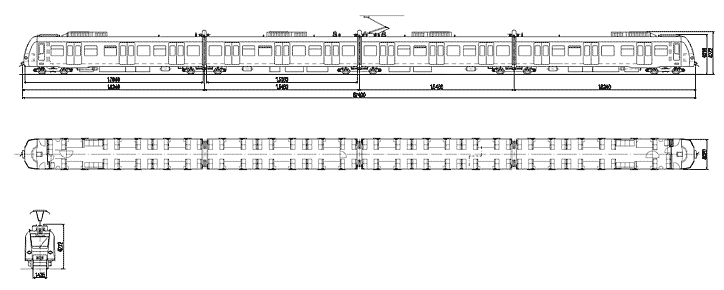
\includegraphics[width=12cm]{et423-techdraw}
  \caption[Technical drawing of \sbahntype.]%
  {Technical drawing of \sbahntype.
    \citefig{http://de.bombardier.com/}{et-423-electric multiple
  unit-techdraw.gif}{}{2016-07-22}}
  \label{fig:et423-techdraw}
\end{figure}

\begin{figure}[htb]
  \centering
  
\includegraphics[width=12cm]{et423-draw}
  \caption[Drawing of \sbahntype.]%
  {Drawing of \sbahntype. The measured part is between the 5th and 6th door.
    \citefig{https://commons.wikimedia.org/}{}{CC BY-SA 3.0}{2016-07-22}}
  \label{fig:et423-draw}
\end{figure}

\begin{figure}[htb]
  \centering
  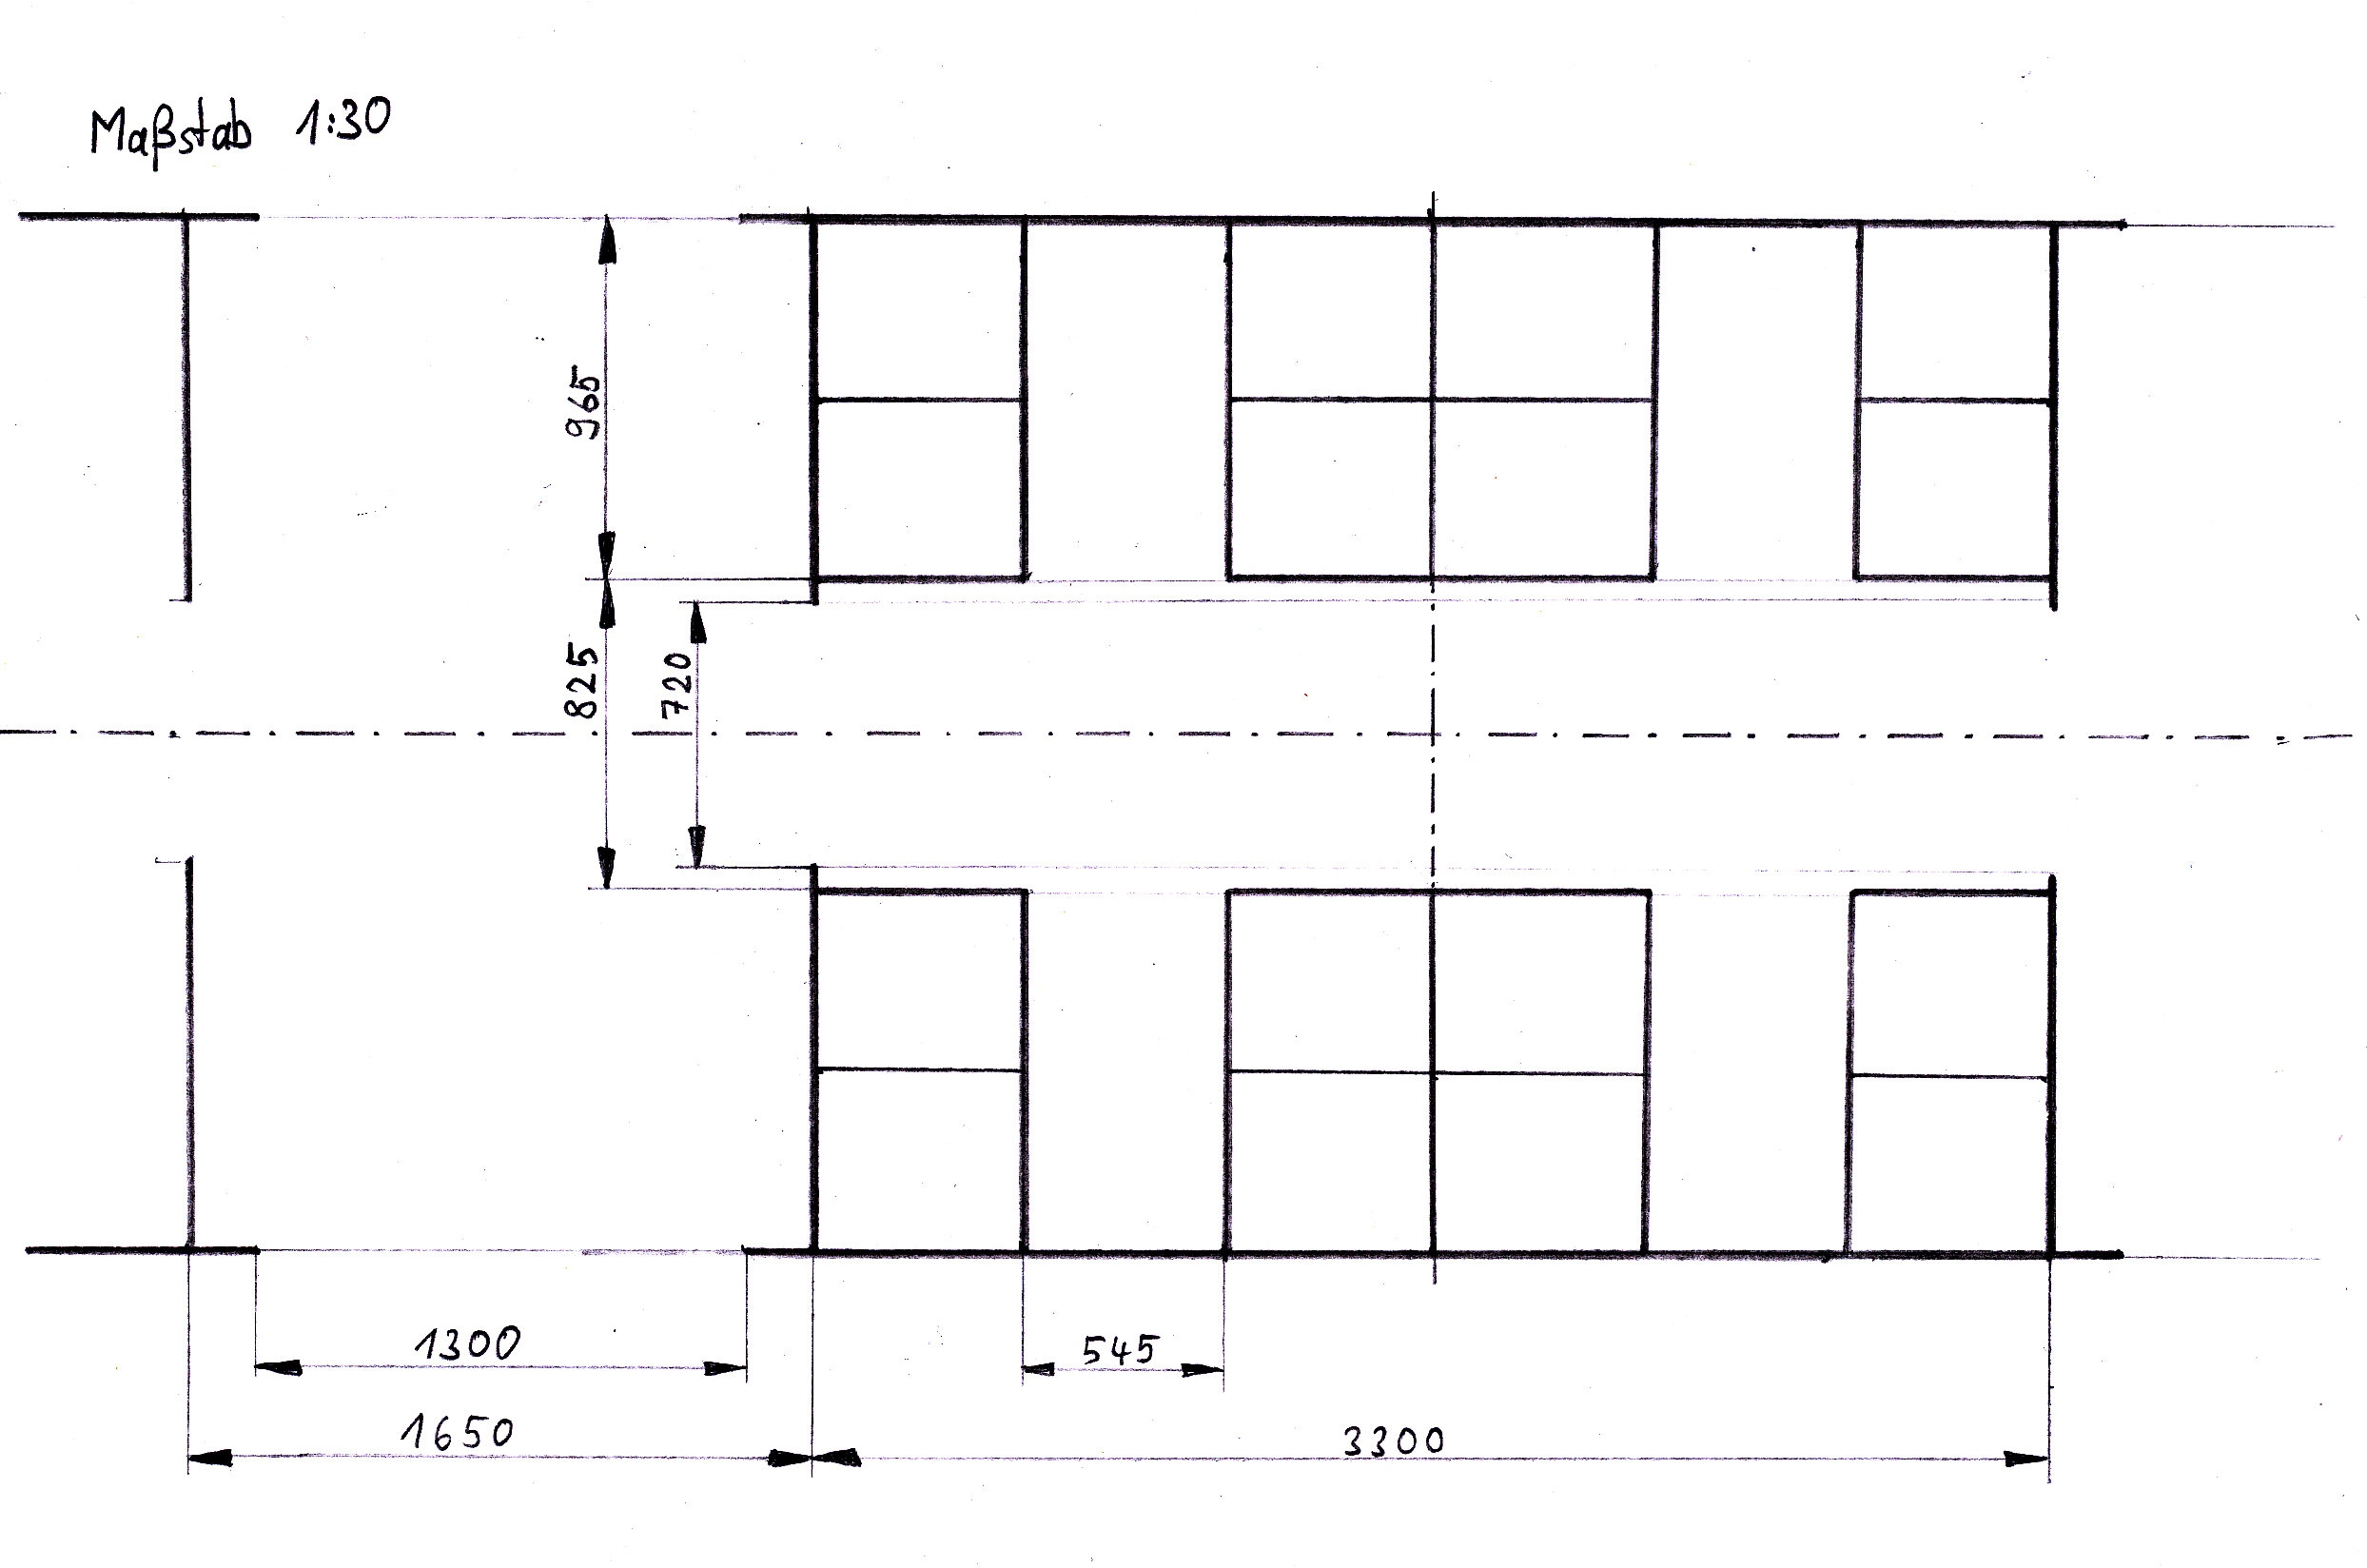
\includegraphics[width=12cm]{et423-techdraw-interior}
  \caption[Technical drawing of the interior of \sbahntype.]%
  {Technical drawing of the interior of \sbahntype.
    Measures were taken at the 5th and 6th entrance area and at the compartment
    inbetween.}
  \label{fig:et423-techdraw-interior}
\end{figure}

\FloatBarrier

\subsection{Usage}

\traingen\ can be started from the \acs{IDE} or from the command line.
When started from the \acs{IDE}, the command line arguments have to be set
there.
In Eclipse, this is done via \emph{Run → Run Configurations} in the
\emph{Arguments} tab.

When started from the command line, the wrapper script \code{traingen.sh} can be
used.
It lets Java run the \traingen\ \acs{JAR} file and passes all given command
line arguments to it.

The scenario file can then be imported into the \vaderegui\ and viewed or edited
in the \emph{Topography Designer} tab (see
figure~\ref{fig:screenshot-scenario-import} and~\ref{fig:screenshot-scenario}).

\begin{figure}[htb]
  \centering
  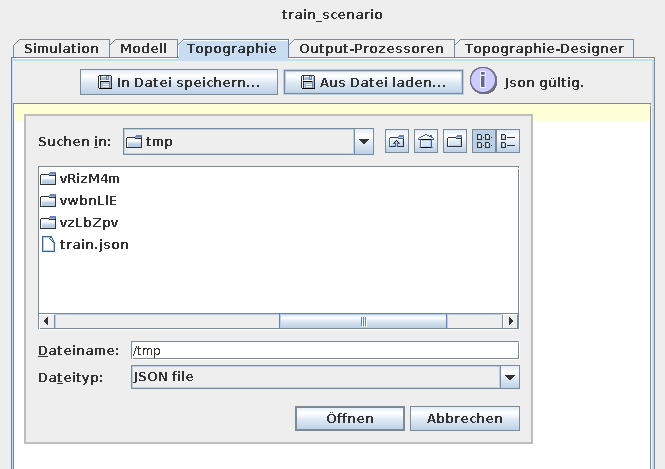
\includegraphics[width=14cm]{screenshot-scenario-import}
  \caption[Import of a scenario file into the \vaderegui.]{%
    Import of a scenario file into the \vaderegui.
    It is done in the \emph{Topography} tab by clicking at the \emph{Load from
    file} button and then selecting a scenario file in \acs{JSON} format.
  }\label{fig:screenshot-scenario-import}
\end{figure}

\begin{figure}[htb]
  \centering
  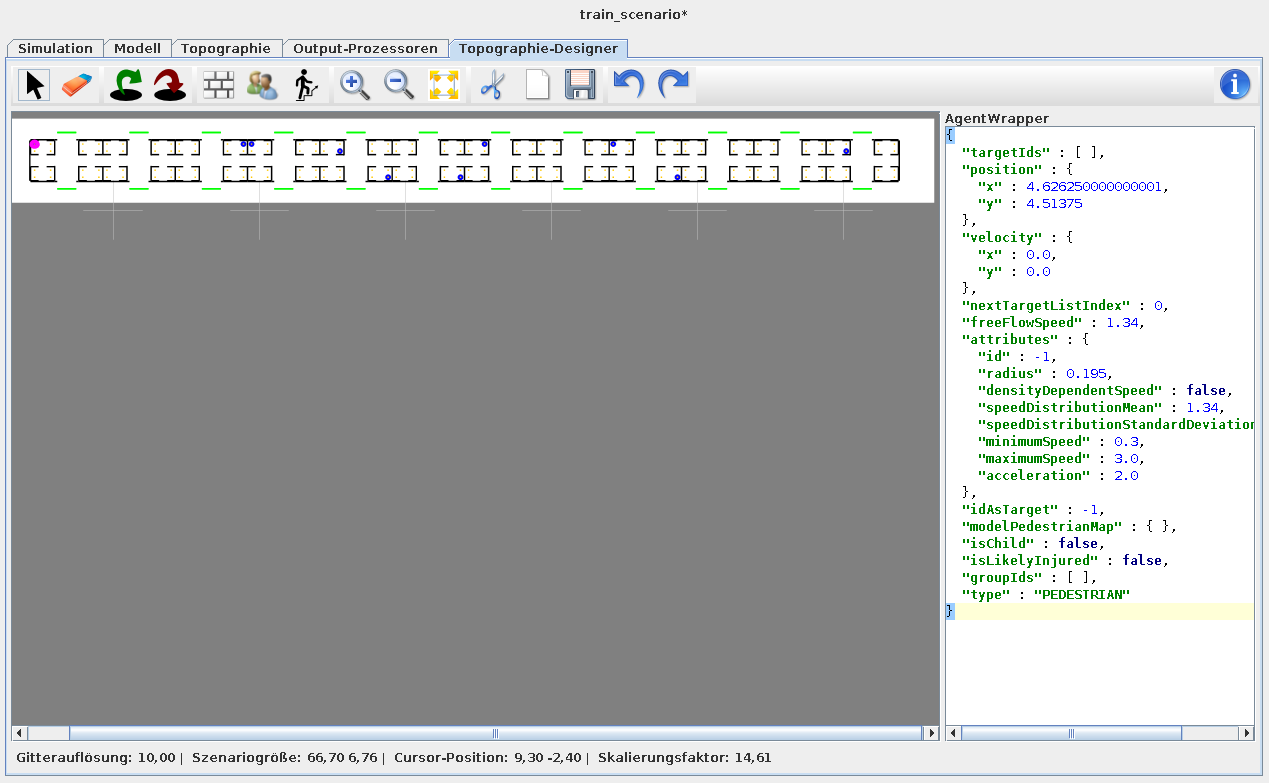
\includegraphics[width=14cm]{screenshot-scenario}
  \caption[A train scenario opened in the \emph{Topography Designer} tab.]{%
  A train scenario opened in the \emph{Topography Designer} tab of the
  \vaderegui.
  }\label{fig:screenshot-scenario}
\end{figure}

\FloatBarrier

\section{Model implementation}
\label{sec:model-implementation}

This section describes the implementation of the seating model in \vadere.
The seating model itself is described in chapter~\ref{ch:model}.

\subsection{Overview}

Simulation models in \vadere\ have to implement the \code{Model} interface
which defines a common interface for initialization.
Models also have to implement the \code{ActiveCallback} interface.
% active callback or model?
This interface declares an \code{update} method (amongst others) which is
repeatedly called from \vadere's main simulation loop.
More details on this are provided in section~\ref{sec:simulation-model-framework}.

\begin{figure}[htb]
  \centering
  \includegraphics[width=8cm]{seatingmodel}
  \caption[Simplified \acs{UML} class diagram of the seating model implementation.]{%
  Simplified \acs{UML} class diagram of the seating model implementation.
  }\label{fig:uml-seatingmodel}
\end{figure}

Figure~\ref{fig:uml-seatingmodel} shows a high-level overview of the seating
model implementation.
The class \code{SeatingModel} implements the interfaces \code{Model} and
\code{ActiveCallback} and has the following instance variables:

\begin{itemize}[noitemsep,nolistsep]

  \item An attributes object which contains the model parameters.
    These parameters can be configured via \acs{JSON} in the scenario file or
    from the \vaderegui.

  \item A \code{TrainModel} object which is a model of the train.
    It is built from the topography and can be viewed as a higher-level wrapper
    class.
    It provides access to compartments, seat groups, seats, and the persons
    sitting on the seats.

  \item A seeded random number generator used for statistical modeling of
    seating decisions.

\end{itemize}

The attributes, the topography, and the random number generator are passed from
\vadere\ to the \code{initialize} method.

\subsection{Implementation}

The model's algorithm is explained in chapter~\ref{ch:model}.
The following is a short outline of what is done for a single person:

\begin{enumerate}[noitemsep]

  \item \label{itm:seating-algo-step1} For a new person entering the train,
    choose a compartment and assign it as target to the person.

  \item \label{itm:seating-algo-step2} For a person arriving in its target compartment, choose a seat group and
    a seat and assign it as target to the person.

  \item \label{itm:seating-algo-step3} For a person arriving at its seat, update the seat object in the train
    model accordingly.

\end{enumerate}

The \code{update} method (listing~\ref{lst:seating-model-update}) is only
concerned about step~\ref{itm:seating-algo-step1}.
For those persons that have no target assigned, it assigns a compartment as
target.
This is a polling approach which slows down the simulation.
A cleaner and more efficient way would be to introduce source listeners in
\vadere, similar to the target listeners introduced in
section~\ref{subsec:target-listener}.
For now, the existing facilities are used.

\lstinputlisting[%
language={Java},%
caption={[The seating model's \code{update} method.]%
  The seating model's \code{update} method which is hooked into the simulation loop.},%
label={lst:seating-model-update}]%
{listings/seating-model-update.java}

The next two steps of the algorithm are implemented using target listeners.
Each compartment and each seat is a target and gets a listener registered in the
\code{initia\-lize} method.

For step~\ref{itm:seating-algo-step2}, a target listener is registered on every
compartment target.
Once a person arrives in its compartment, the listener implementation chooses
and assigns a seat as the new target.

For step~\ref{itm:seating-algo-step3}, a target listener is registered on every
seat target.
Once a person arrives at its seat, the train model's seat object is updated to
reference the now sitting person.

Special cases are not described in this section.
Instead, they are identified and described in
section~\ref{subsec:model-special-cases} and implemented accordingly.

\subsection{Tests}

The seating model is tested with \href{http://junit.org/junit4/}{JUnit~4} unit
tests.
There are currently 72 % TODO Number of runs (test methods) when starting AllSeatingModelRelatedTests
test methods which cover 52\% of the \code{SeatingModel} class and 98\% of the
related train model classes on which the seating model builds upon (branch
coverage, \citep{myers2004art}).\footnote{
  The Eclipse plugin \href{http://www.eclemma.org/}{EclEmma~2.3.3} was used to
  measure code coverage.}
There is a JUnit test suite to combine all tests related to the
seating model in a hierarchical way which allows for running all related tests
together.

\section{Model verification}
\label{sec:model-verification}

The basic idea for a higher-level verification of the seating model is letting
the simulation generate the same kind of data as that from the data collection.
The real and the simulated data can then be compared which is described in
chapter~\ref{ch:evaluation}.
This section describes how the data is generated in the simulation.

In \vadere, the data processor subsystem is used to generate data during a
simulation.
Data processors aggregate, process, and store data about the simulation.
They are hooked into the simulation loop---similar to
\code{ActiveCallback}s (section~\ref{sec:simulation-model-framework}).
When the simulation is finished, the aggregated data is written to output files
in a table format, \eg \acs{CSV}.
A more detailed documentation of this subsystem can be found in the \vadere\
repository in the \emph{Documentation} folder.

The data processor for verification is called \code{LogEventProcessor} because it
produces the same data format as the log-event data from the survey (see
section~\ref{subsec:data-format} and table~\ref{tab:logevent-data-columns}).
However, only sit-down events are recorded in the simulation; other events are
not needed for verification.

Involved classes are \code{LogEventProcessor},
\code{AttributesLogEventProcessor}, \code{Log\-Event\-OutputFile}, \code{IdDataKey},
and \code{LogEventEntry}.
The latter two classes are used in key-value pairs to store the data in the
processor.
\code{LogEventEntry} represents one logged event in the output file.

The logic is implemented in the \code{LogEventProcessor} class:

\begin{itemize}

  \item During initialization, the class reads its attributes (the compartment
    to observe, the survey \acs{ID} to use, and the initial value for the person
    \acs{ID} counter).
    It also gets the \code{TrainModel} instance from the seating model to obtain
    access to compartments and seats.
    It then registers a target listener\footnote{See
    section~\ref{subsec:target-listener} for details.} on all seats in the
    assigned compartment.

  \item Before the simulation starts, the processor sets an instance variable to
    the current time.
    During the simulation, this time variable is updated and used as timestamp
    for the logged events.
    For persons already sitting in the train, the processor stores initial
    sit-down events and then the ``initialization end'' event.
    These events are not considered in the data analysis but capture the initial
    situation in the train.

  \item During the simulation, the time variable is periodically updated in the
    \code{doUp\-date} method.
    Asynchronously, the target listener is called when a person sits down on a
    seat.
    This sit-down event is then stored in the processor's key-value store.

\end{itemize}

After the simulation, the \code{LogEventOutputFile} writes the aggregated data
to disk.
Because the processor is parameterized with its
\code{AttributesLogEvent\-Proces\-sor}, multiple compartments can be observed during
one single simulation.
The output files from multiple simulations can also be combined to one single
dataset.
The resulting dataset is used in chapter~\ref{ch:evaluation} to verify the
seating model.

\section{Summary}

I presented some aspects of design, implementation, and development of the
mobile app for data collection and discussed a different architectural approach.

I introduced \vadere, an existing simulation framework for pedestrian dynamics,
and I presented enhancements and new features.
New modules have been carefully designed around the simulator without invading
or bloating existing core modules.
Shortcomings in the software design have been located and fixed.
I also introduced coding standards and contribution guidelines for the \vadere\
open source project which help to ensure code quality.

I implemented a new simulation model in \vadere\ to simulate people's seating
behavior in \sbahn\ trains, and I integrated a system to verify the simulation
by comparing its output to real data from a data collection.
I developed a tool to auto-generate train scenarios with a variety of options.
These scenarios are not restricted to seating model applications but can be used
in other areas of research on pedestrian dynamics as well.
